% !TEX root = sum1.tex
\section{Results}
We carried out several experiments, including analyzing the performances of different policies, evaluating the impact of implementing social distancing.

% assessing the results for different numbers of people in each period and finally investigating the impact of seat layout on the number of served people.

\subsection{Performances of Different Policies}
In this section, we compare the performance of five dynamic seat assignment policies to the optimal value, which can be obtained by solving the deterministic model after observing all arrivals. The policies under examination are the stochastic planning policy, DP Base-heuristic, bid-price control, booking limit control and FCFS policy. 


% dynamic programming based heuristic and booking limit control. Finally, we establish the FCFS policy as the benchmark.

\subsubsection*{Numerical Results}
The seat layout consists of 10 rows, each with 21 seats (including one dummy seat as the social distance), and the group size can range up to 4 people. We conducted experiments over 60 to 100 periods to demonstrate the policies' performance under varying demand levels. We selected three probabilities to ensure that the expected number of people for each period is consistent. The table below displays the average of 200 instances for each number.

An arrival sequence during $T$ periods can be expressed as ${y_1, y_2, \ldots, y_T}$. Let $N_i = \sum_{t} I(y_t = i)$, i.e., the count number of times group type $i$ arrives during $T$ periods. Then the scenarios, $(N_1, \ldots, N_M)$, follow a multinomial distribution, 
$$
p\left(N_1, \ldots, N_M \mid \mathbf{p}\right)=\frac{T !}{N_{1} !, \ldots, N_{M} !} \prod_{i=1}^M p_i^{N_i}, T=\sum_{i=1}^M N_i.
$$

It is clear that the number of different sequences is $M^T$. The number of different scenarios is
$O(T^{M-1})$ which can be obtained by the following DP. The number of scenarios is too large to enumerate all possible cases. Thus, we choose to sample some sequences from the multinomial distribution.


\begin{table}[ht]
  \centering
  \caption{Performances of Different Policies}
  \begin{tabular}{|l|l|l|l|l|l|l|}
  \hline
   T & probabilities & DSA (\%) & DP1 (\%) & Bid-price (\%) & Booking (\%) & FCFS (\%) \\
  \hline
   60  & [0.25, 0.25, 0.25, 0.25]  & 99.12 & 98.42 & 98.38 & 96.74 & 98.17 \\
   70  &                           & 98.34 & 96.87 & 96.24 & 97.18 & 94.75 \\
   80  &                           & 98.61 & 95.69 & 96.02 & 98.00 & 93.18 \\
   90  &                           & 99.10 & 96.05 & 96.41 & 98.31 & 92.48 \\
   100 &                           & 99.58 & 95.09 & 96.88 & 98.70 & 92.54 \\
   \hline
   60  & [0.25, 0.35, 0.05, 0.35]  & 98.94 & 98.26 & 98.25 & 96.74 & 98.62 \\
   70  &                           & 98.05 & 96.62 & 96.06 & 96.90 & 93.96 \\
   80  &                           & 98.37 & 96.01 & 95.89 & 97.75 & 92.88 \\
   90  &                           & 99.01 & 96.77 & 96.62 & 98.42 & 92.46 \\
   100 &                           & 99.23 & 97.04 & 97.14 & 98.67 & 92.00 \\
  \hline
  60  & [0.15, 0.25, 0.55, 0.05]  & 99.14 & 98.72 & 98.74 & 96.61 & 98.07 \\
  70  &                           & 99.30 & 96.38 & 96.90 & 97.88 & 96.25 \\
  80  &                           & 99.59 & 97.75 & 97.87 & 98.55 & 95.81 \\
  90  &                           & 99.53 & 98.45 & 98.69 & 98.81 & 95.50 \\
  100 &                           & 99.47 & 98.62 & 98.94 & 98.90 & 95.25 \\
  \hline
  \end{tabular}
\end{table}

We can find that the stochastic planning policy are better than DP Base-heuristic and bid-price policy consistently, and FCFS policy works worst. As we mentioned previously, DP Base-heuristic and bid-price policy can only make the decision to accept or deny, cannot decide which row to assign the group to. FCFS accepts groups in sequential order until the capacity cannot accommodate more.


For the first three policies, their performance tends to initially drop and then increase as the number of periods increases. When the number of periods is small, the demand for capacity is relatively low, and the policies can achieve relatively optimal performance. However, as the number of periods increases, the policies may struggle to always obtain a perfect allocation plan, leading to a decrease in performance. Nevertheless, when the number of periods continue to become larger, these policies tend to accept larger groups, and as a result, narrow the gap with the optimal value, leading to an increase in performance.

%  当之前的上座率 小于 gamma/gamma+1, 制定社交距离没有影响
%  大于 gamma/gamma+1, 则最大损失是( )

\subsection{Impact of Implementing Social Distancing in DSA}
In this section, our focus is to analyze the influence of social distancing on the number of accepted individuals. Intuitively, when demand is small, we will accept all arrivals, thus there is no difference whether we implement the social distancing. What is interesting for us is when the difference occurs. Our primary objective is to determine the first time period at which, on average, the number of people accepted without social distancing is not less than the number accepted with social distancing plus one. This critical point, referred to as the gap point, is of interest to us. Additionally, we will examine the corresponding occupancy rate at this gap point. It should be noted that the difference at a specific time period may vary depending on the total number of periods considered. Therefore, when evaluating the difference at a particular time period, we assume that there are a total of such periods under consideration.


It is evident that as the demand increases, the effect of social distancing becomes more pronounced. We aim to determine the specific time period where the absence of social distancing results in a higher number of accepted individuals compared to when social distancing measures are in place. Additionally, we will calculate the corresponding occupancy rate during this period.

By analyzing and comparing the data, we can gain insights into the relation between demand, social distancing, the number of accepted individuals, and occupancy rates. This information is valuable for understanding the impact of social distancing policies on overall capacity utilization and making informed decisions regarding resource allocation and operational strategies.

\subsubsection{Estimation of Gap Point}
% Based on our findings, we observed that the seat allocation derived from the optimal solution consistently satisfies the formation of either the largest pattern or the full pattern, regardless of different probability combinations. 

% We can leverage the expected number of people in each period to estimate the gap point when utilizing the DSA. 

% We can approximate the period at which the number of people accepted without social distancing surpasses the number accepted with social distancing, based on the performance characteristics observed in the DSA.

% However, certain counterexamples arise when the requirements associated with specific probability combinations are unable to form a full pattern, resulting in gaps in the seating arrangement. The occurrence of these counterexamples is closely tied to the seat layout itself. 


% Given the stable gap between the seat assignment policy obtained from SPP and the optimal policy, 
To find such a first period, we aim to find the maximum period such that we could assign all the groups during these periods into the seats, i.e., for each group type $i$, we have $\sum_{j} x_{ij} \geq d_i$, where $x_{ij}$ is the number of group type $i$ in row $j$. Meanwhile, we have the capacity constraint $\sum_{i} n_{i} x_{ij} \leq L_j$, thus, $\sum_{i} n_i d_i \leq \sum_{i} n_i \sum_{j} x_{ij} \leq \sum_{j} L_{j}$. Notice that $E(d_i) = p_i T$, we have $\sum_{i} n_i p_i T \leq \sum_{j} L_{j}$ by taking the expectation. Let $L = \sum_{j} L_{j}$, representing the total number of seats, $\gamma = \sum_{i} i p_i$, representing the average number of people who arrive in each period, we can obtain $T \leq \frac{L}{\gamma + \delta}$, then the upper bound of the expected maximum period is $T' = \frac{L}{\gamma + \delta}$.

% To find such a first period, we aim to find the maximum period such that we could assign all the groups during these periods into the seats, i.e., for each group type $i$, we have $\sum_{j} x_{ij} \geq d_i$, where $x_{ij}$ is the number of group type $i$ in row $j$. Meanwhile, we have the capacity constraint $\sum_{i} n_{i} x_{ij} \leq L_j$, thus, $\sum_{i} n_i d_i \leq \sum_{i} n_i \sum_{j} x_{ij} \leq \sum_{j} L_{j}$. Notice that $E(d_i) = p_i T$, we have $\sum_{i} n_i p_i T \leq \sum_{j} L_{j}$ by taking the expectation. Let $L = \sum_{j} L_{j}$, representing the total number of seats, $\gamma = \sum_{i} i p_i$, representing the average number of people who arrive in each period, we can obtain $T \leq \frac{L}{\gamma + \delta}$, then the upper bound of the expected maximum period is $T' = \frac{L}{\gamma + \delta}$.

Assuming that we accept all incoming groups within $T'$ periods, filling all the available seats, the corresponding occupancy rate at this period can be calculated as $\frac{\gamma T'}{(\gamma+ \delta)T' - N \delta} = \frac{\gamma}{\gamma +\delta} \frac{L}{L-N \delta}$. However, it is important to note that the actual maximum period will be smaller than $T{'}$ because it is impossible to accept groups to fill all seats exactly. To estimate the gap point when applying DSA, we can use $y_1 = c_1 \frac{L}{\gamma + \delta}$, where $c_1$ is a discount rate compared to the ideal assumption. Similarly, we can estimate the corresponding occupancy rate as $y_2 = c_2 \frac{\gamma}{\gamma +\delta} \frac{L}{L-N \delta}$, where $c_2$ is a discount rate for the occupancy rate compared to the ideal scenario.

% Assuming that we accept all incoming groups within $T'$ periods, filling all the available seats, the total number of people, taking social distancing into account, would be equal to the number of all seats. This can be expressed as $\gamma T' + \delta T' = L$, where $\gamma T'$ is the expected number of people. Thus, the expected period for reaching this point is given by $T' = \frac{L}{\gamma + \delta}$.


% It is important to note that this estimation is accurate only when we accepted groups in $T{'}$ periods and all rows represent full patterns, as per our assumption. 
% $T{'}$ represents the ideal first period where the number of people without social distancing is larger than that with social distancing 

We consider the scenario where the number of group types is limited to 4. In this case, the average number of people per period, denoted as $\gamma$, can be expressed as $\gamma = p_1 \cdot 1 + p_2 \cdot 2 + p_3 \cdot 3 + p_4 \cdot 4$, where $p_1$, $p_2$, $p_3$, and $p_4$ represent the probabilities of groups with one, two, three, and four people, respectively. We assume that $p_4$ always has a positive value. Additionally, the social distancing requirement is set to one seat.

To analyze the relation between the increment of $\gamma$ and the gap point, we define each combination $(p_1, p_2, p_3, p_4)$ satisfying $p_1 + p_2 + p_3 + p_4 = 1$ as a probability combination. We conducted an analysis using a sample of 200 probability combinations. The figure below illustrates the gap point as a function of the increment of $\gamma$, along with the corresponding estimations. For each probability combination, we considered 100 instances and plotted the gap point as blue points. Additionally, the occupancy rate at the gap point is represented by red points.

To provide estimations, we utilize the equations $y_1 = \frac{c_1 L}{\gamma + \delta}$(blue line in the figure) and $y_2 = c_2 \frac{\gamma}{\gamma + \delta} \frac{L}{L-N \delta}$(orange line in the figure), which are fitted to the data. These equations capture the relation between the gap point and the increment of $\gamma$, allowing us to approximate the values. By examining the relation between the gap point and the increment of $\gamma$, we can find that $\gamma$ can be used to estimate gap point.

\begin{figure}[ht]
  \centering
    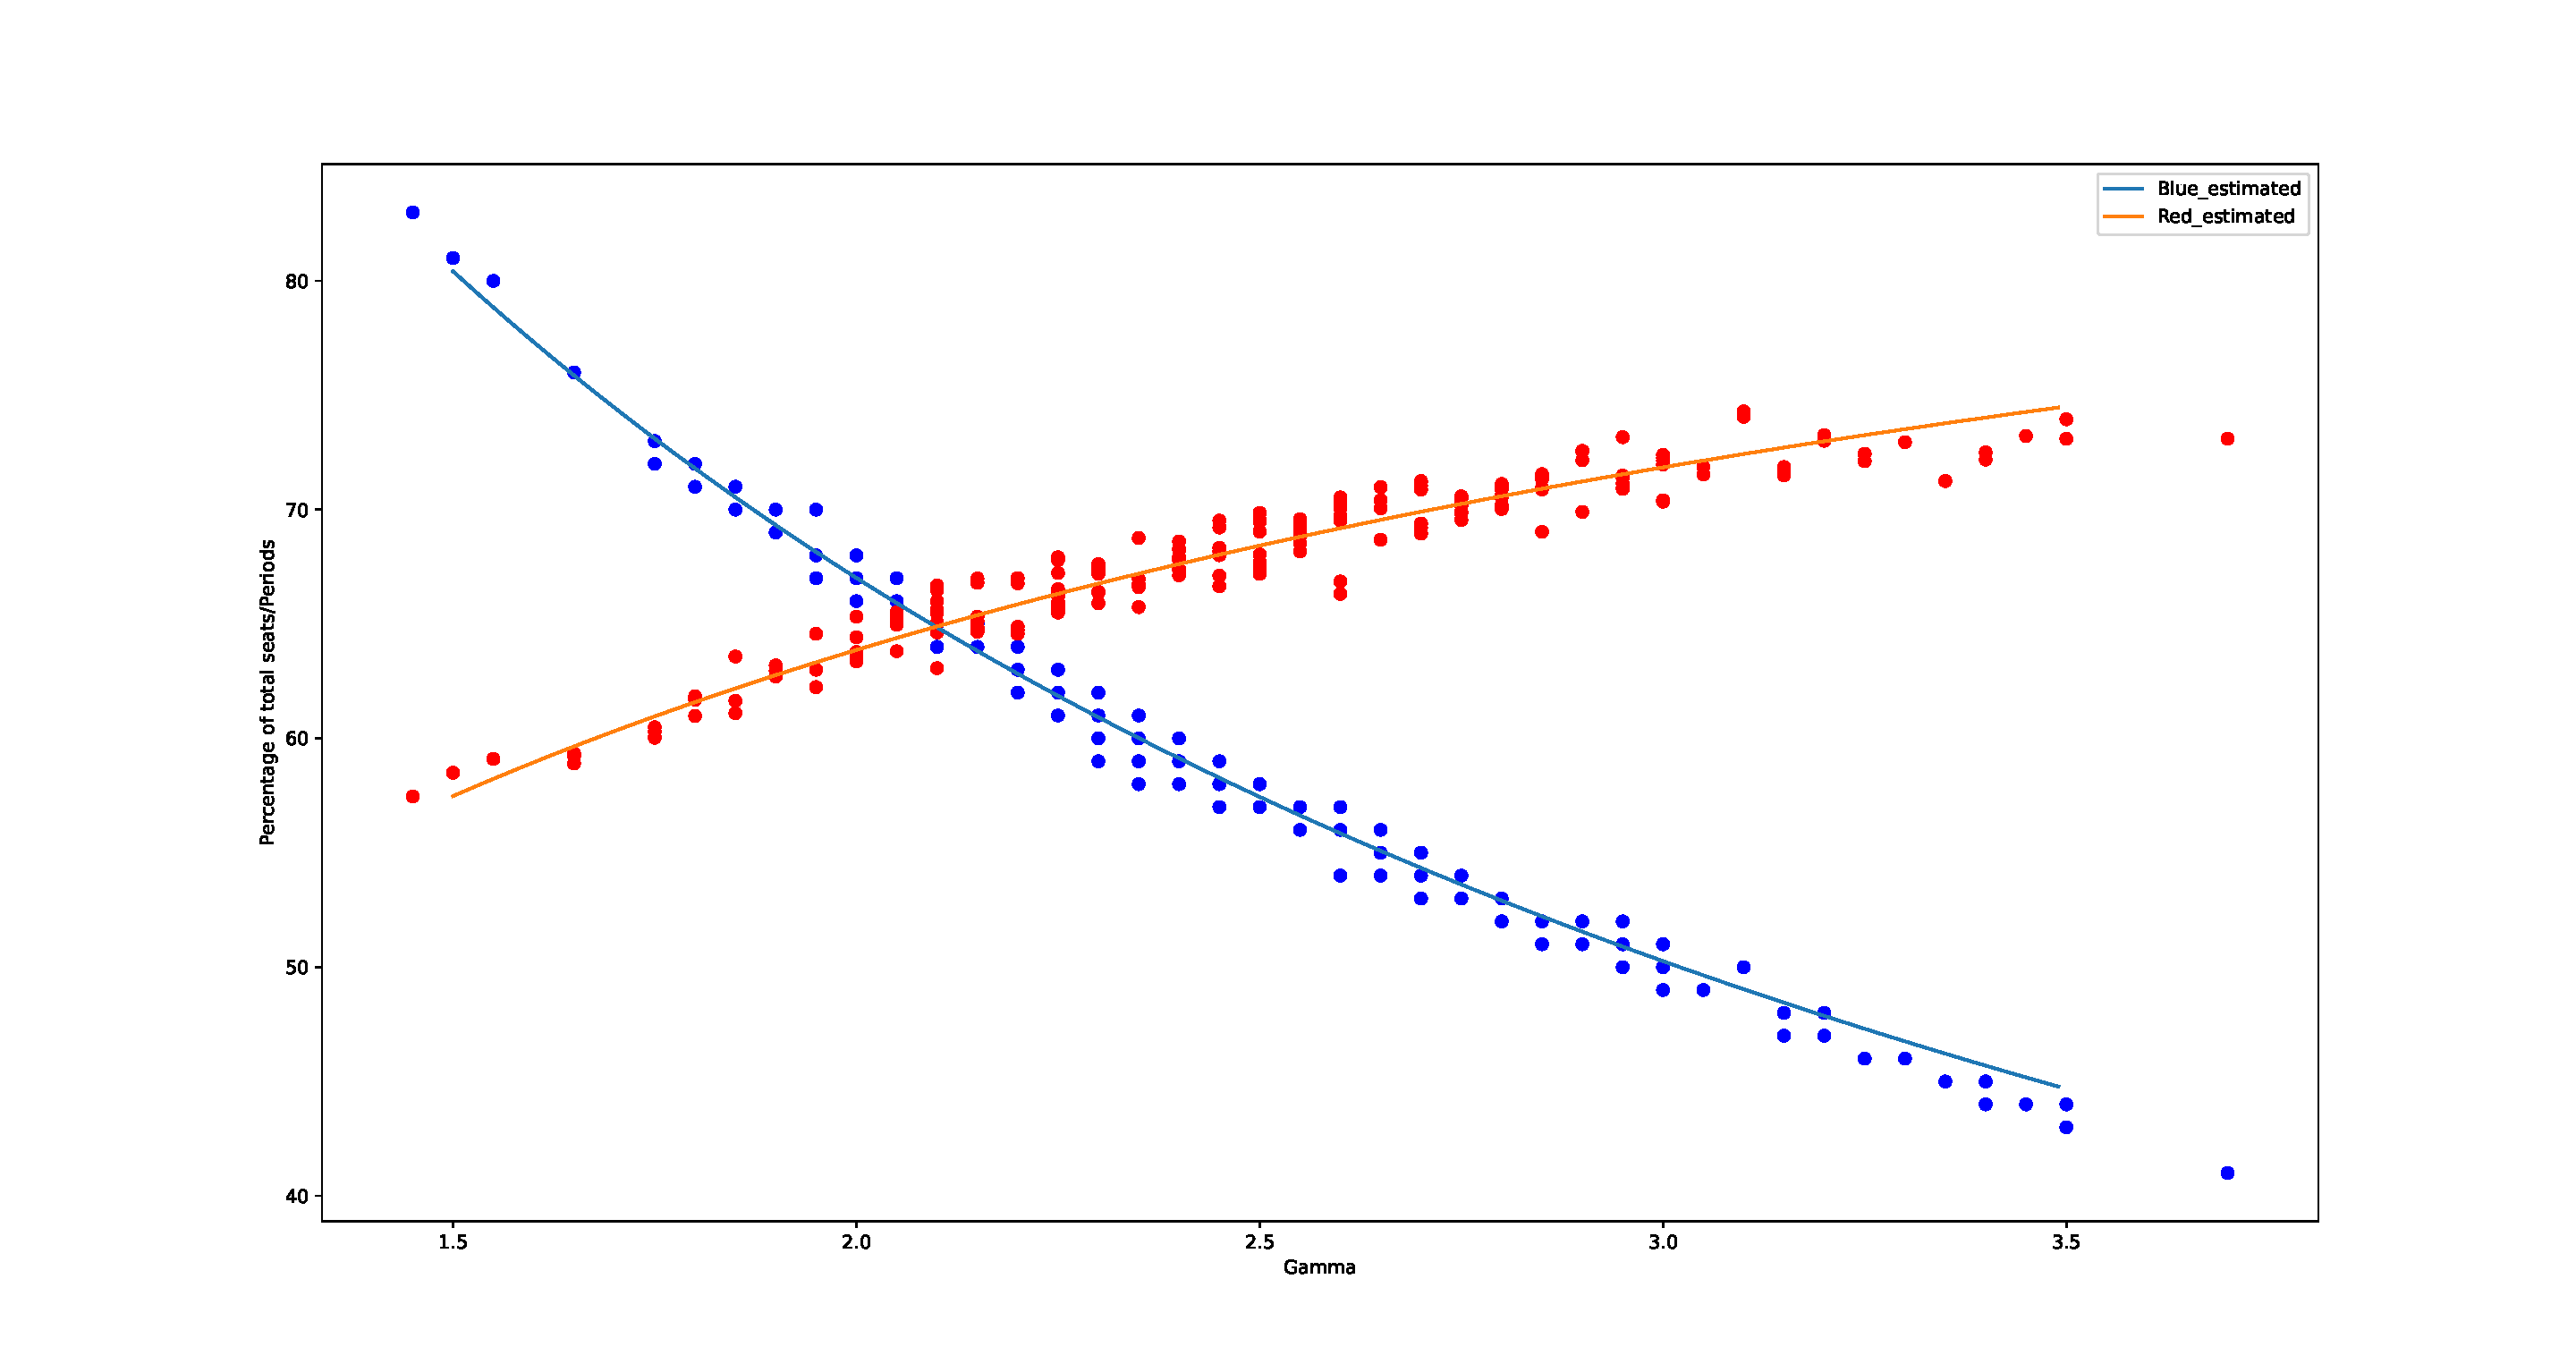
\includegraphics[width=0.8\textwidth]{./Figures/re2.pdf}
  \caption{Gap points and their estimation under 200 probabilities}
\end{figure}

% For the first function, we found that $c_1 = 200.0208$, with a standard error of 0.203. For the second function, we obtained $c_2 = 90.9284$, with a standard error of 0.099. 


The estimation of $c_1$ and $c_2$ can be affected by different seat layouts. To investigate this impact, we conduct several experiments using different seat layouts, specifically with the number of rows $\times$ the number of seats configurations set as 10 $\times$ 16, 10 $\times$ 21, 10 $\times$ 26 and 10 $\times$ 31. Similarly, we perform an analysis using a sample of 100 probability combinations, each with a mean equal to $\gamma$. The values of $\gamma$ range from 1.5 to 3.4. We employed an Ordinary Least Squares (OLS) model to fit the data and derive the parameter values. The goodness of fit is assessed using the R-square values, which are found to be 1.000 for all models, indicating a perfect fit between the data and the models.

The results of the estimation of $c_1$ and $c_2$ are presented in the table below:

\begin{table}[ht]
  \centering
  \caption{Estimation of $c_1$ and $c_2$}
  \begin{tabular}{|c|c|c|}
  \hline
   Seat layout(\# of rows $\times$ \# of seats) & Estimation of $c_1$ & Estimation of $c_2$  \\
  \hline
   10 $\times$ 11 & 0.909 $\pm$ 0.013  & 89.89 $\pm$ 1.436 \\
   10 $\times$ 16 & 0.948 $\pm$ 0.008  & 94.69 $\pm$ 0.802 \\
   10 $\times$ 21 & 0.955 $\pm$ 0.004 & 95.44 $\pm$ 0.571 \\
   10 $\times$ 26 & 0.966 $\pm$ 0.004 & 96.23 $\pm$ 0.386 \\
   10 $\times$ 31 & 0.965 $\pm$ 0.003 & 96.67 $\pm$ 0.434 \\
   10 $\times$ 36 & 0.968 $\pm$ 0.003 & 97.04 $\pm$ 0.289 \\
   \hline
  \end{tabular}
\end{table}


% when the probability combination is $[0.05, 0.05, 0.85, 0.05]$ (which corresponds to $\gamma = 2.9$), and the demands cannot be accommodated by constructing full patterns for every row, which does not satisfy our assumption. This leads to a considerable gap between the blue and red points in this case. For example, the demands could be $[4, 1, 45, 2]$ or $[2, 2, 47, 1]$ according to the probability combination, but the typical pattern that can be generated is $(4,4,4,4)$, which is not full.


\subsubsection{Impact of Social Distancing as Demands Increase}
Now, we consider the impact of social distance as demands increase by changing $T$. Specifically, we consider two situations: $\gamma = 1.9$ and $\gamma = 2.5$. We set the parameters as follows: $T$ varies from 30 to 120, the step size is 1.  The seat layout consists 10 rows and the number of seats per row is 21. The social distancing is 1 seat.

The figure below displays the outcomes of groups who were accepted under two different conditions: with social distancing measures and without social distancing measures. For the former case, we employ DSA to obtain the results. In this case, we consider the constraints of social distancing and optimize the seat allocation accordingly. For the latter case, we adopt a different approach. We simply accept all incoming groups as long as the capacity allows, without considering the constraints of groups needing to sit together. This means that we prioritize filling the available seats without enforcing any specific seating arrangements or social distancing requirements. We conduct an analysis using a sample of 100 probability combinations associated with the same $\gamma$. The occupancy rate at different demands is calculated as the mean of these 100 samples. The figures depicting the results are presented below.

% Since the various probabilities with the same $\gamma$ exhibit similar patterns as shown in the figure, we present only one case of probabilities to illustrate the detailed figure.

\begin{figure}[h]
  \centering
  \subfigure[When $\gamma =1.9$]{
    \label{Fig.sub.1}
    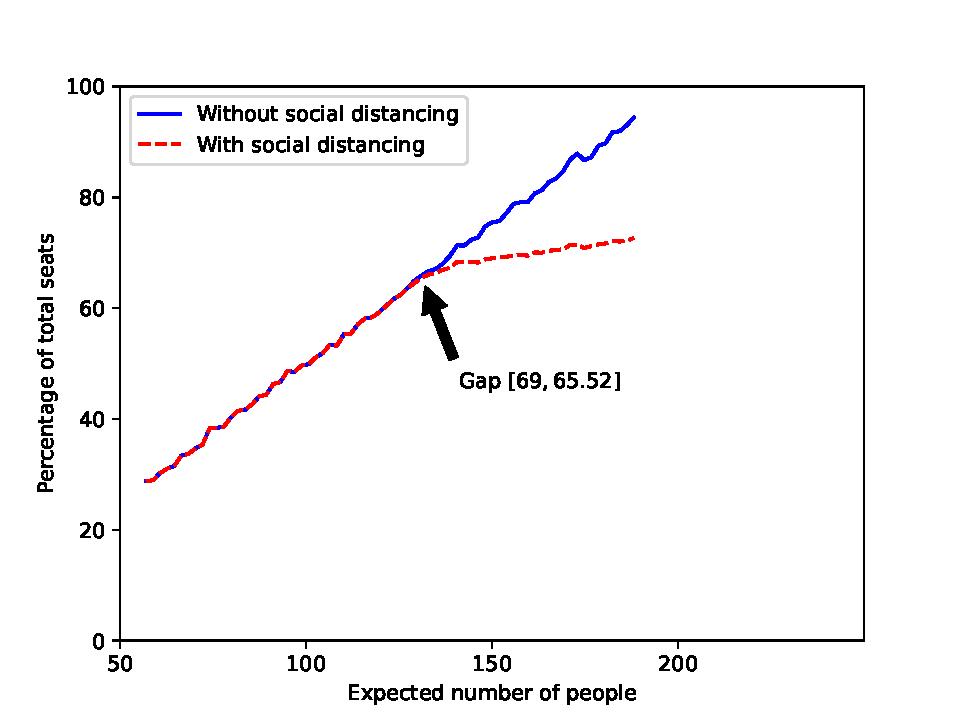
\includegraphics[width=0.48\textwidth]{./Figures/p2.pdf}}
  \subfigure[When $\gamma =2.5$]{
    \label{Fig.sub.2}
    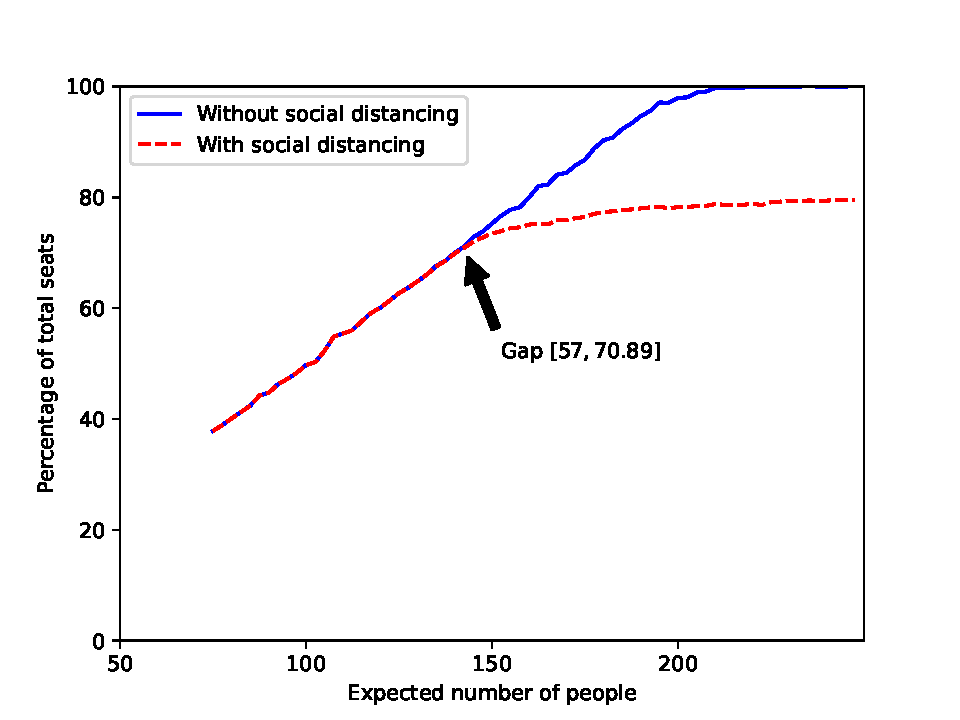
\includegraphics[width=0.48\textwidth]{./Figures/p1.pdf}}
  \caption{The occupancy rate over the number of arriving people}
  \label{Fig.lable}
\end{figure}

The analysis consists of three stages. 
In the first stage, when the capacity is sufficient, the outcome remains unaffected by the implementation of social distancing measures. In the second stage, as the value of $T$ increases, the difference between the outcomes with and without social distancing measures becomes more pronounced. Finally, in the third stage, as $T$ continues to increase, both scenarios reach their maximum capacity acceptance. At this point, the gap between the outcomes with and without social distancing measures begins to converge. For the social distancing situation, according to Proposition \ref{lem_pattern}, when the largest pattern is assigned to each row, the resulting occupancy rate is $\frac{16}{20} = 80\%$, which is the upper bound of occupancy rate.

% The maximum number of people that can be accepted is $200 * \frac{16}{20} = 160$, which is the upper bound on the number of people that can be accepted.

The below table presents the percentage differences for different demand levels (130, 150, 170, 190, 210).

% \begin{table}[ht]
%   \centering
%   \caption{Percentage differences under different demands}
% \begin{tabular}{llllll}
%   \hline
%   \multicolumn{1}{|l|}{\multirow{2}{*}{$\gamma$}}  &  \multicolumn{5}{l|}{Percentage gaps under different demands}   \\ 
%   \cline{2-6} 
%   \multicolumn{1}{|l|}{}   & \multicolumn{1}{l|}{130} & \multicolumn{1}{l|}{150} & \multicolumn{1}{l|}{170} & \multicolumn{1}{l|}{190} & \multicolumn{1}{l|}{210} \\ 
%   \hline
%   \multicolumn{1}{|l|}{1.9} &   \multicolumn{1}{l|}{0.27}  & \multicolumn{1}{l|}{6.39}  & \multicolumn{1}{l|}{13.23} & \multicolumn{1}{l|}{21.85} & \multicolumn{1}{l|}{25.69} \\
%   \hline
%   \multicolumn{1}{|l|}{2.1} &   \multicolumn{1}{l|}{0.27}  & \multicolumn{1}{l|}{6.39}  & \multicolumn{1}{l|}{13.23} & \multicolumn{1}{l|}{21.85} & \multicolumn{1}{l|}{25.69} \\
%   \hline
%   \multicolumn{1}{|l|}{2.3} &   \multicolumn{1}{l|}{0.27}  & \multicolumn{1}{l|}{6.39}  & \multicolumn{1}{l|}{13.23} & \multicolumn{1}{l|}{21.85} & \multicolumn{1}{l|}{25.69} \\
%   \hline      
%   \multicolumn{1}{|l|}{2.5}   & \multicolumn{1}{l|}{0}  & \multicolumn{1}{l|}{1.46}  & \multicolumn{1}{l|}{9.23} & \multicolumn{1}{l|}{17.32} & \multicolumn{1}{l|}{21.59} \\ 
%   \hline
%   \multicolumn{1}{|l|}{2.7} &   \multicolumn{1}{l|}{0.27}  & \multicolumn{1}{l|}{6.39}  & \multicolumn{1}{l|}{13.23} & \multicolumn{1}{l|}{21.85} & \multicolumn{1}{l|}{25.69} \\
%   \hline  
% \end{tabular}
% \end{table}

\begin{table}[ht]
  \centering
  \caption{Gap points and percentage differences under different demands of different gammas}
\begin{tabular}{lllllll}
  \hline
  \multicolumn{1}{|l|}{\multirow{2}{*}{$\gamma$}} & \multicolumn{1}{l|}{\multirow{2}{*}{gap point}} & \multicolumn{5}{l|}{percentage differences under different demands}   \\ 
  \cline{3-7} 
  \multicolumn{1}{|l|}{}                      & \multicolumn{1}{l|}{}                    & \multicolumn{1}{l|}{130} & \multicolumn{1}{l|}{150} & \multicolumn{1}{l|}{170} & \multicolumn{1}{l|}{190} & \multicolumn{1}{l|}{210} \\ 
  \hline
  \multicolumn{1}{|l|}{1.9}  & \multicolumn{1}{l|}{[69, 65.52]}  & \multicolumn{1}{l|}{0.25}  & \multicolumn{1}{l|}{5.82}  & \multicolumn{1}{l|}{12.82} & \multicolumn{1}{l|}{20.38} & \multicolumn{1}{l|}{24.56} \\ 
  \hline                                    
  \multicolumn{1}{|l|}{2.1}  & \multicolumn{1}{l|}{[64, 67.74]}  & \multicolumn{1}{l|}{0.05}  & \multicolumn{1}{l|}{4.11}  & \multicolumn{1}{l|}{11.51} & \multicolumn{1}{l|}{18.77} & \multicolumn{1}{l|}{21.87} \\ 
  \hline           
  \multicolumn{1}{|l|}{2.3}  & \multicolumn{1}{l|}{[61, 69.79]}  & \multicolumn{1}{l|}{0}  & \multicolumn{1}{l|}{2.29}  & \multicolumn{1}{l|}{10.21} & \multicolumn{1}{l|}{17.36} & \multicolumn{1}{l|}{21.16} \\ 
  \hline           
  \multicolumn{1}{|l|}{2.5}  & \multicolumn{1}{l|}{[57, 70.89]}  & \multicolumn{1}{l|}{0}  & \multicolumn{1}{l|}{1.45}  & \multicolumn{1}{l|}{9.30} & \multicolumn{1}{l|}{15.78} & \multicolumn{1}{l|}{19.80} \\ 
  \hline          
  \multicolumn{1}{|l|}{2.7}  & \multicolumn{1}{l|}{[53, 71.28]}  & \multicolumn{1}{l|}{0}  & \multicolumn{1}{l|}{1.38}  & \multicolumn{1}{l|}{7.39} & \multicolumn{1}{l|}{14.91} & \multicolumn{1}{l|}{19.14} \\ 
  \hline            
\end{tabular}
\end{table}


As the value of $\gamma$ increases, the period of gap point will decrease and the corresponding occupancy rate will Increase. This suggests that larger groups are more likely to be accepted, resulting in a smaller number of accepted groups overall. Consequently, the occupancy rate increases due to the allocation of seats to larger groups. The percentage difference is negligible when the demand is small, but it becomes more significant as the demand increases.


Let us consider the scenario where the gap point is defined as $[T, OR]$ under the parameters $\delta$, $\gamma$, and $M$, with the total number of seats denoted as $L$. When the actual number of people (demand) is less than $L \cdot OR$, the implementation of social distancing has no impact on the revenue. However, when the actual number of people exceeds $L \cdot OR$, implementing social distancing will result in a revenue loss. The magnitude of this loss can be determined through simulations using the corresponding parameters. To mitigate this potential loss, the seller can increase the value of $\gamma$. This can be achieved by either setting a limit on the number of single-person groups or allowing for larger group sizes. By doing so, the goal is to minimize the negative impact of social distancing measures and maximize revenue within the constraints imposed by the occupancy rate.


% [0.27 6.39 13.23 21.85 25.69] 1.9
% [ 0.04  4.97 13.55 20.99 24.81] 2
% [0 1.46 9.23 17.32 21.59] 2.5

% \subsection{Comparison of Different Probabilities When Supply and Demand Are Close}
% When we set the number of periods $T$ to be equal to $T'$, representing a state where the expected demand and supply are in balance, we can observe differences among the outcomes for different probabilities.

% We sample $p_1$, $p_2$, and $p_3$ from 0.05 to 0.95 with an increment of 0.05. The seat layout still remains the same as the above experiments. The figure below shows the number of people served for each value of $\gamma$. For each probability combination, the blue point represents the average number of people served over 50 instances, and the red point represents the estimated number of people served. 

% \begin{figure}[h]
%   \centering
%   \subfigure[One instance for each probability combination]{
%     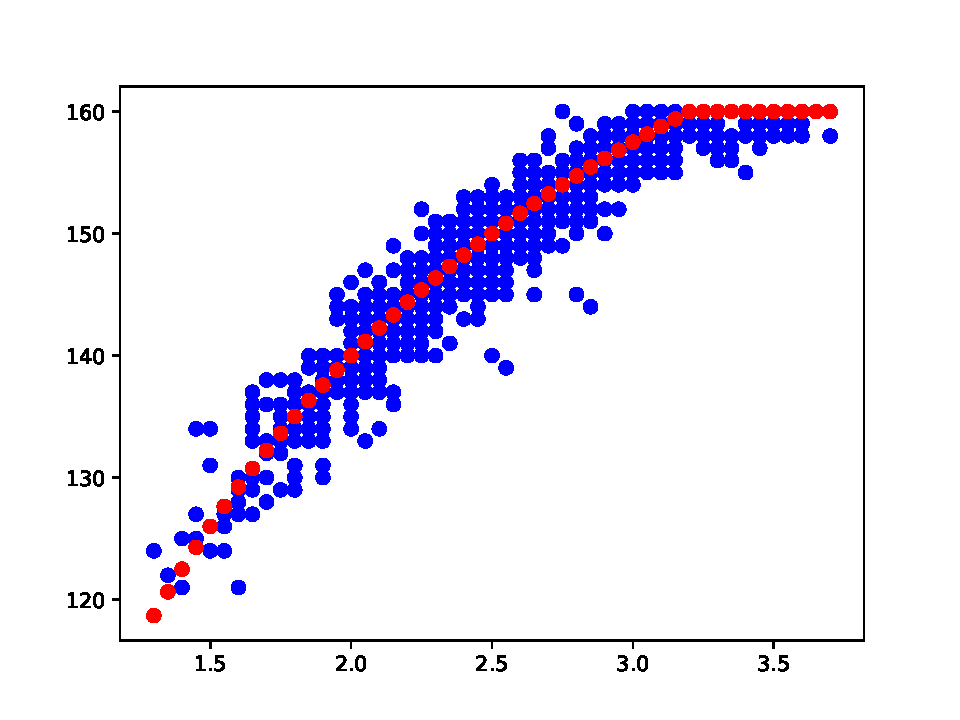
\includegraphics[width=0.48\textwidth]{./Figures/diff_1.pdf}}
%   \subfigure[Average of 50 instances for each probability combination]{
%     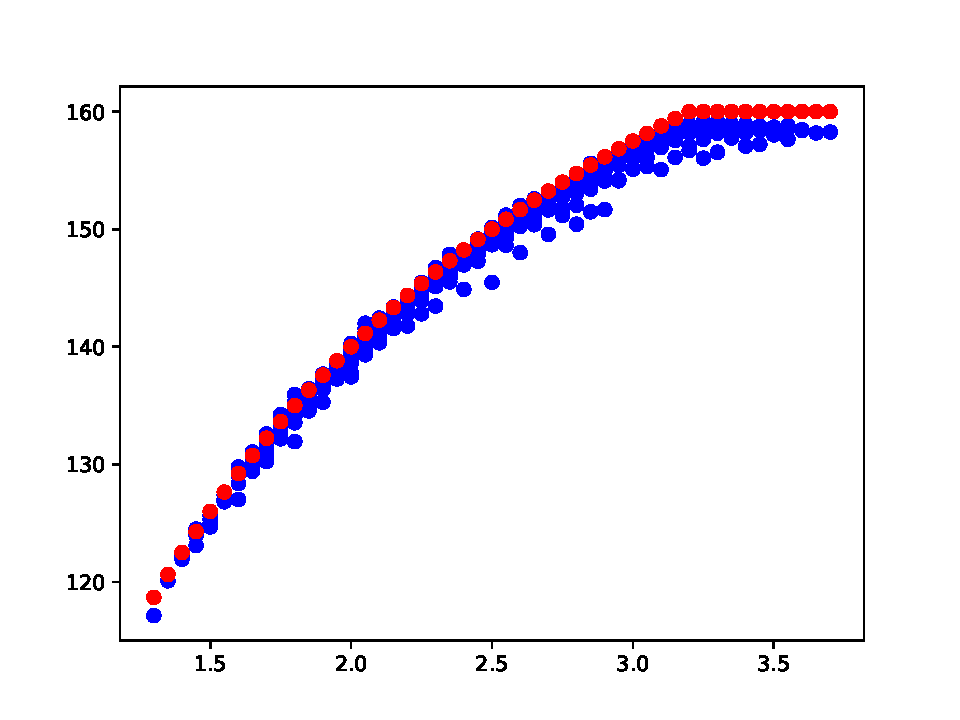
\includegraphics[width=0.48\textwidth]{./Figures/diff_2.pdf}}
%   \caption{The number of people accepted versus $\gamma$}
% \end{figure}

% If the largest pattern is assigned to each row, the resulting occupancy rate is $\frac{16}{21}$. The maximum number of people that can be accepted is $200 * \frac{16}{20} = 160$, which is the upper bound on the number of people that can be accepted. The estimated number of people accepted is given by $\frac{\gamma}{\gamma+1} * 200$, as indicated by the red points in the figure.

% \subsubsection{Analysis on The Difference Between Blue and Red Points}
% We can give the absolute difference between the blue point and red point for each probability combination as below.

% \begin{table}[ht]
%   \centering
%   \caption{Absolute Difference Proportion}\label{tab_diff}
%   \begin{tabular}{|l|l|l|l|l|}
%   \hline
%   \# of instances & abs\_diff $\geq$ 1 & abs\_diff $\geq$ 2 & abs\_diff $\geq$ 3 & abs\_diff $\geq$ 4 \\
%   \hline
%   20 & 32.92 \% & 5.13 \% & 1.74\% & 0.51 \% \\
%   50 & 22.46 \% & 4.31 \% & 1.54 \% & 0.31 \%  \\
%   100 & 20.00 \% & 4.21 \% & 1.54 \% & 0.31 \% \\
%   \hline
%   \end{tabular}
% \end{table}

% \begin{figure}[ht]
%   \centering
%   \subfigure[Average of 50 instances for each probability combination]{
%     \label{Fig1}
%     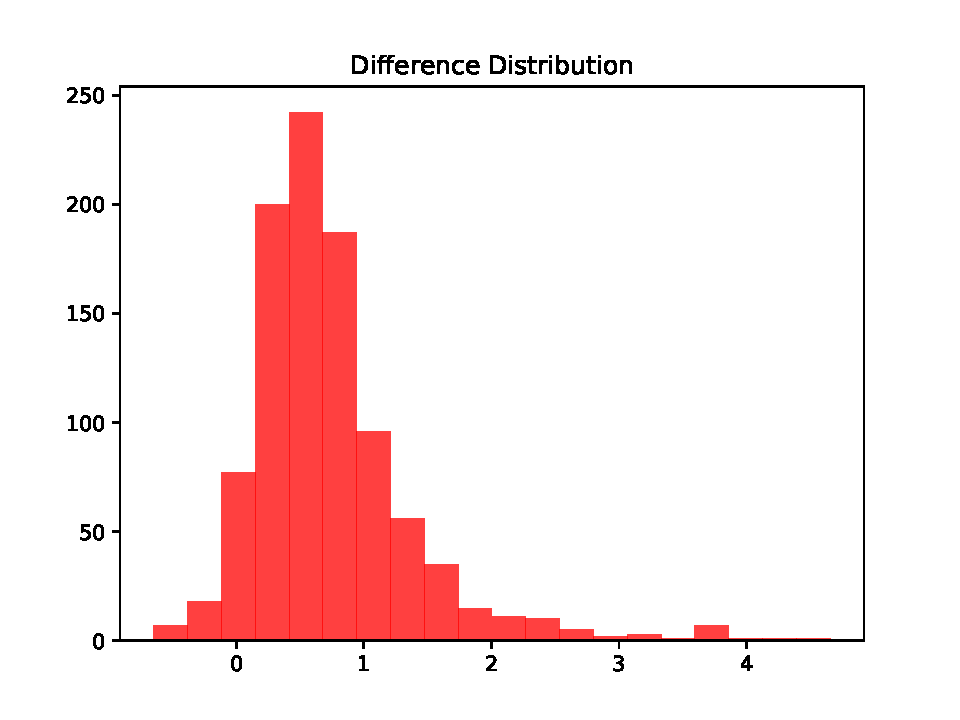
\includegraphics[width=0.48\textwidth]{./Figures/Figure_50.pdf}}
%   \subfigure[Average of 100 instances for each probability combination]{
%     \label{Fig2}
%     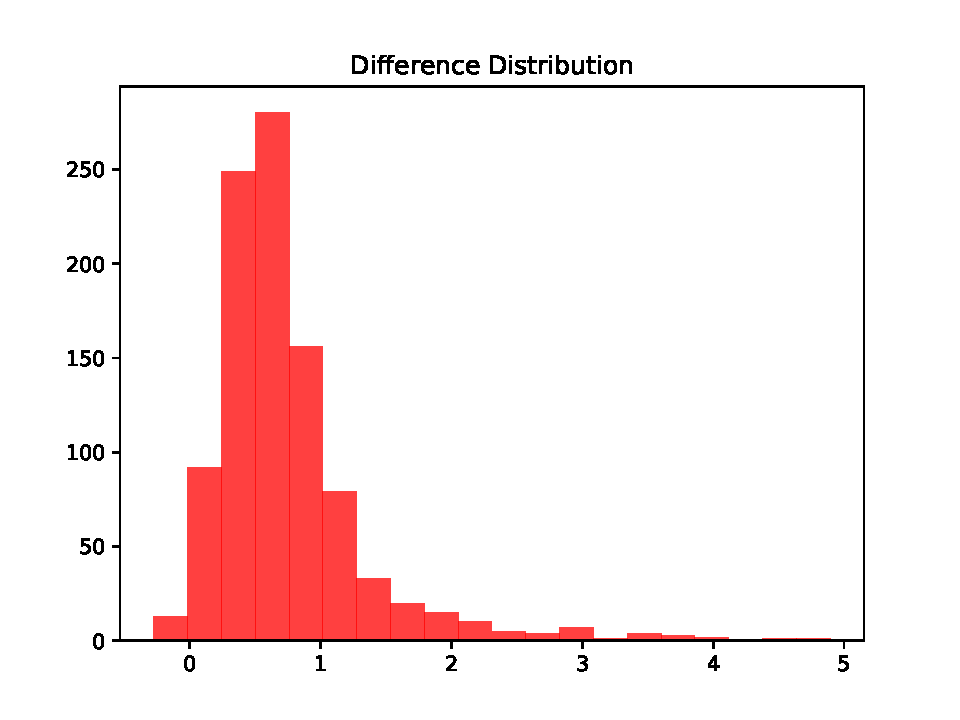
\includegraphics[width=0.48\textwidth]{./Figures/Figure_100.pdf}}
%   \caption{The difference distribution}
%   \label{fig_diff}
% \end{figure}

% Table \ref{tab_diff} displays the absolute difference proportion for the average of 20, 50, and 100 instances, while Figure \ref{fig_diff} shows the difference distribution for the average of 50 and 100 instances. These results suggest that we can estimate the attendance rate based on $\gamma$ for most probability combinations.

% However, we have also observed that some blue points in the figure are significantly distant from their corresponding red points. This is evident when the probability combination is $[0.05, 0.05, 0.85, 0.05]$ (which corresponds to $\gamma = 2.9$), and the demands cannot be accommodated by constructing full patterns for every row, which does not satisfy our assumption. This leads to a considerable gap between the blue and red points in this case. For example, the demands could be $[4, 1, 45, 2]$ or $[2, 2, 47, 1]$ according to the probability combination, but the typical pattern that can be generated is $(4,4,4,4)$, which is not full.


% % \begin{table}[ht]
% %   \centering
% %   \caption{Gap points and gap percentage of different probabilities}
% %   \begin{tabular}{|l|l|l|}
% %   \hline
% %   $\gamma$  & gap point & gap percentage \\
% %   \hline
% %   $[1.5,1.7]$   & [56, ] & [65.21, ] \\
% %   $[1.7,1.9]$   & [56, ] & [65.21, ] \\
% %   $[1.9,2.1]$   & [56, ] & [65.21, ] \\
% %   $[2.1,2.3]$   & [56, ] & [65.21, ] \\
% %   $[2.1,2.3]$   & [56, ] & [65.21, ] \\
% %   \hline
% %   \end{tabular}
% % \end{table}


% % For each $\gamma$, we give several probabilities in the table. We can find the actual gap points with the same $\gamma$ are close.

% % \begin{table}[ht]
% %   \centering
% %   \caption{Actual Gap points of different probabilities}
% %   \begin{tabular}{|l|l|l|l|}
% %   \hline
% %   $\gamma$  & probabilities & gap point & gap percentage \\
% %   \hline
% %   2.5  & [0.25,0.25,0.25,0.25] & 56 & 65.21 \\
% %   2.5  & [0.1,0.4,0.4,0.1] & 55 & 65.59 \\
% %   2.5  & [0.1, 0.5, 0.2, 0.2] & 55 & 65.45 \\
% %   2.5  & [0.2, 0.3, 0.3, 0.2] & 54 & 64.56 \\
% %   2.5  & [0.3, 0.2, 0.2, 0.3] & 55 & 65.51\\
% %   2.5  & [0.2, 0.4, 0.1, 0.3] & 55 & 65.41 \\
% %   1.9  & [0.4, 0.4, 0.1, 0.1] & 67 & 60.35 \\
% %   1.9  & [0.5, 0.2, 0.2, 0.1] & 67 & 58.9  \\
% %   1.9  & [0.3, 0.5, 0.2, 0]  &  68 & 61.7  \\
% %   1.9  & [0.6, 0.1, 0.1, 0.2] & 66 & 58.31 \\
% %   \hline
% %   \end{tabular}
% % \end{table}


% % \subsubsection{Results of Different Seat Layouts}
% % If we modify the even seat layout, the differences between the red and blue points will decrease, and some outliers may be eliminated. To maintain the same total seating capacity, we compare two layouts with the even seat layout. The step-size seat layout consists of rows with 17, 18, 19, 20, 21, 21, 22, 23, 24, and 25 seats, while the random seat layout has rows with 19, 20, 21, 21, 23, 24, 26, 17, 19, and 20 seats. Both layouts can accommodate a maximum of 164 people when each row corresponds to the largest pattern.

% % \begin{figure}[ht]
% %   \centering
% %   \subfigure[Average of 50 instances for step-size seat layout]{
% %     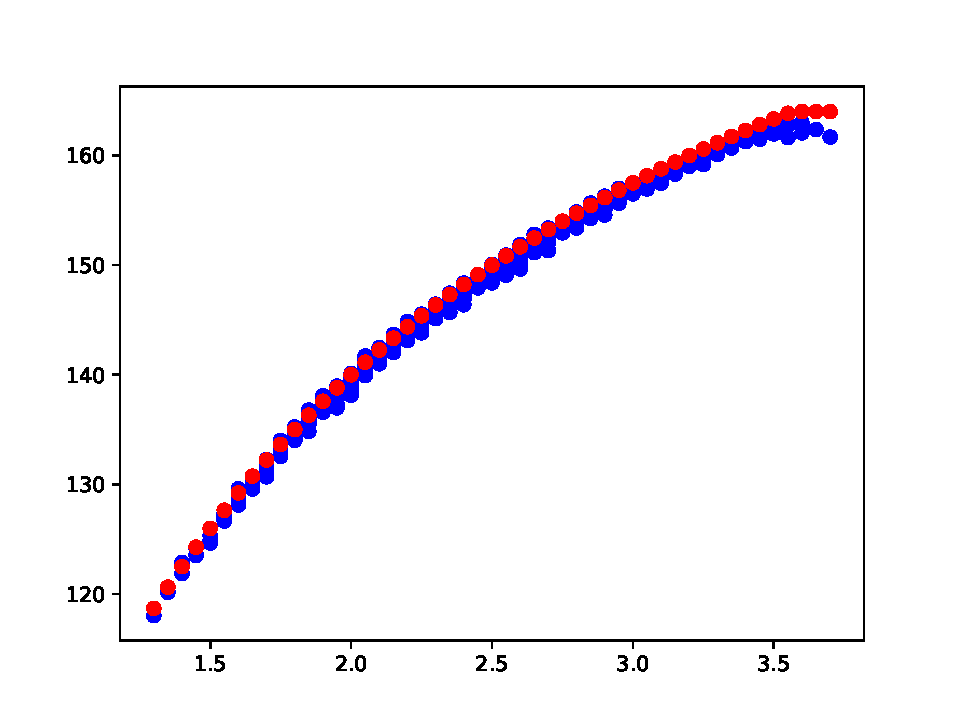
\includegraphics[width=0.48\textwidth]{./Figures/stepsize_seat.pdf}}
% %   \subfigure[Average of 50 instances for random seat layout]{
% %     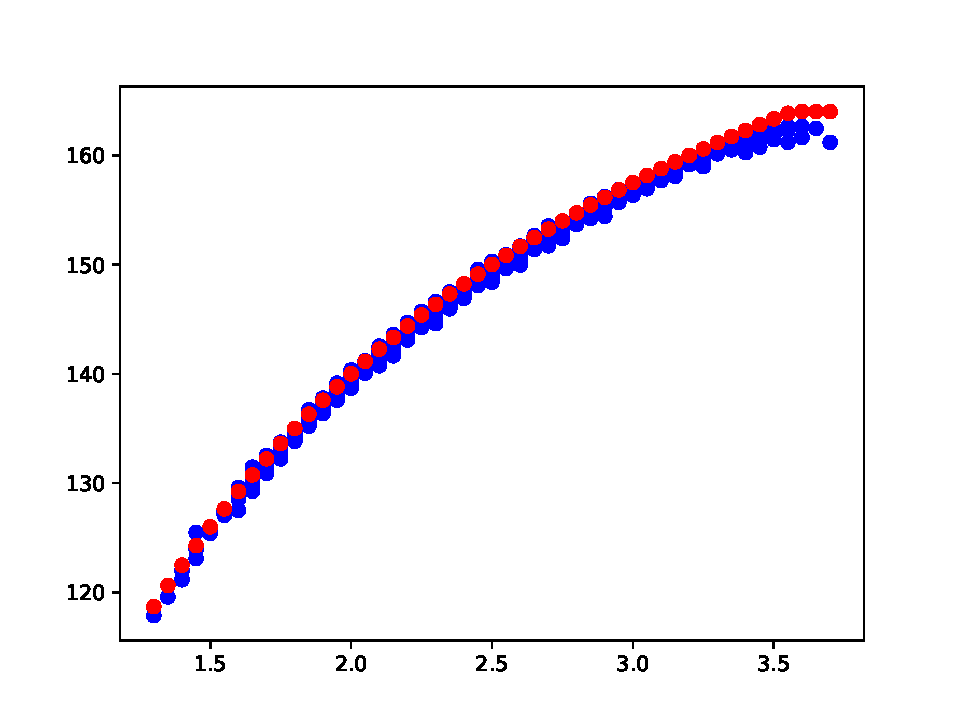
\includegraphics[width=0.48\textwidth]{./Figures/random_seat.pdf}}
% %   \caption{The number of people served versus $\gamma$}
% % \end{figure}

% % The results suggest that a random seat layout may provide a more accurate estimation, implying that such a layout is more capable of accommodating uncertain demands and achieving a full pattern that can accept more people.

% % % When $p = [0.25, 0.25, 0.25, 0.25]$, $E(D) = 2.5 T$. Let $p_1*1 + p_2*2 + p_3*3 + p_4*4 = 2.5$, 
% % % Let $E(D) = 150, T = 50, 60, 75$. The number of seats: 200, 210, 225.


% % \newpage

% % % In addition, we evaluate two policies for seat assignment after all group arrivals: one is based on dynamic programming (DP) and the other is based on first-come, first-served (FCFS) scheduling.
% % % We present the results of our experiments and discuss their implications.


% \subsection{Measurement}
% Suppose a real scenario with a fixed sequence, $s^{r}$. Solving the following program can obtain the optimal value, $V_{s^{r}}$. (Offline)

% Then the difference is $V_{s^{r}} - \text{our result}$.

% WS(the value under wait-and-see policy with all possible scenarios)

% EVPI(Expected Value of Perfect Information) = WS - the value of deterministic equivalent form
